% SUPERSEDED on 2026-10-30 by "results - circuit-level noise.tex". This file is not included in main.tex.
\subsection{LRB-D under SI1000 Noise}
\label{sub:si1000_results}

We next benchmark the folded $[[5,1,2]]_3$ patch under the qutrit SI1000 noise model of \autoref{subsub:si1000_model}. The protocol is unchanged from \autoref{sub:simulation_results}. Each stabilizer generator is measured with its own ancilla, so the simulated system consists of nine qutrits, five data and four ancillas. We sweep 15 raw noise strengths $p$ from $0$ to $0.05$, corresponding to normalized strengths $\lambda = 5p$ from $0$ to $0.25$, with logical depths up to $m=22$ and $10^6$ shots per depth spread over 30 independent random Clifford sequences. These runs are sampled through the compiled detector error model backend of \autoref{sec:sdim-dem}, which is what makes this shot count affordable across the full grid of check schedules.

The physical reference is single-qutrit RB with the depolarizing channel $\mathcal{E}_{\mathcal{D}}(p_{RB})$ applied after every Clifford, simulated at $p_{RB} = \lambda$ on the matching grid with $10^4$ shots per depth. Since $\lambda$ is the flip rate on each ancilla readout, the worst single location in the encoded circuit, the comparison asks whether an encoded qutrit whose worst location fails at rate $\lambda$ can outperform a bare qutrit that suffers that same rate at every gate.

\subsubsection{Terminal post-selection}
In the terminal regime no stabilizer checks are inserted during the sequence, and the accept or reject decision is made only once, from the terminal $X$-basis data readout by evaluating the two $X$-type stabilizers on the recorded outcomes. \autoref{fig:si1000_terminal} shows the resulting traces. The LRB-D curves again fail to follow a single exponential, with a flat shoulder at small depth followed by a faster decay, which is the same multi-mode syndrome memory discussed in \autoref{sub:irreps}. For this reason we extract no fit parameters in the terminal regime. Compared to the depolarizing results of \autoref{fig:sim_terminal_nofit}, however, the departure is visibly milder, and the encoded traces now sit above the matched physical baseline across the entire sweep. The reason is the SI1000 rate hierarchy. Between checks the logical Cliffords only pick up single-qutrit noise at rate $p/10 = \lambda/50$ and entangling noise at rate $\lambda/5$, so at a fixed value of the noise coordinate the encoded sequence accumulates far less error than the depolarizing model injects, while the physical baseline is held at the full rate $\lambda$ per gate.

\begin{figure}[H]
  \centering
  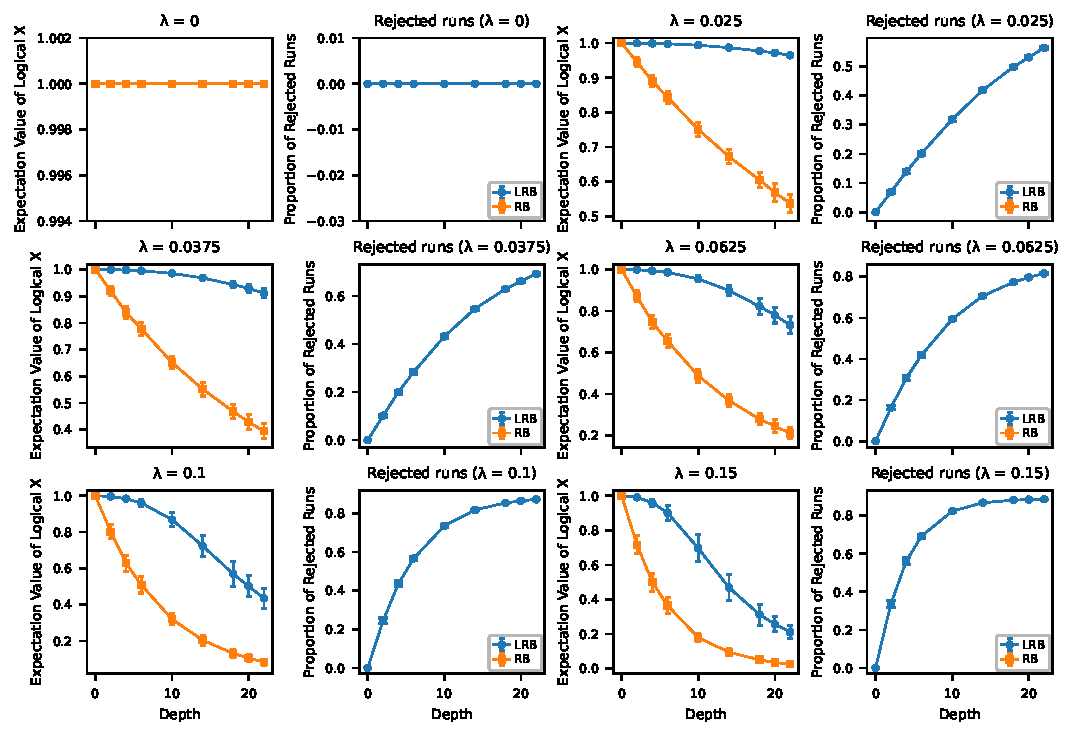
\includegraphics[width=0.95\textwidth]{
    figures/si1000-const-0-Summary-Graph-NoFit.pdf}
  \caption{Terminal post-selection under qutrit SI1000 noise. We pick out six representative values of $\lambda$ up to $0.15$. Columns 1 and 3: $\langle \bar{X}\rangle$ versus logical depth for LRB-D (blue) compared to the $\langle X \rangle$ physical RB baseline at $p_{RB}=\lambda$ (orange). Columns 2 and 4: fraction of rejected shots versus depth. The LRB-D traces remain non-exponential, but the deviation is milder than in the depolarizing model and the encoded qutrit retains an advantage over the matched physical baseline throughout.}
  \label{fig:si1000_terminal}
\end{figure}

\subsubsection{Uniform-interval post-selection}
We then apply uniform-interval post-selection, checking all four stabilizers every $k$ logical Cliffords and rejecting a shot as soon as any check returns a non-trivial outcome. All fitting in this section is confined to these interval-check runs. For each $k$ we fit the accepted-shot survival curves to the decay model of Eq.~\eqref{eq:fseq} with the offset fixed to $B = 0$, following the convention of \autoref{sub:simulation_results}. The physical RB baseline is fit with the same zero-offset model, and fidelities are extracted through Eq.~\eqref{eq:fbar}.

\paragraph{Near-Markovian limit ($k=1$).}
As in the depolarizing case, checking after every logical Clifford collapses the dynamics back toward a two-mode structure, and the decay curves in \autoref{fig:si1000_unif1_fit} are well described by a single exponential. The encoded advantage below threshold is substantial. At $\lambda = 0.025$ we extract an average logical gate fidelity of $\bar{F} = 0.9993$ against a physical $\bar{F} = 0.9814$, and at $\lambda = 0.1$ we obtain $0.9710$ against $0.9288$. By $\lambda = 0.15$ the two are statistically indistinguishable, at $0.8980$ against $0.8965$, which is consistent with the pseudo-threshold extracted below. The cost of this regime is that every check layer now carries its own noise. Each of the four ancilla readouts flips at rate $5p = \lambda$, so a sizable fraction of shots is rejected by the very first check layer even at depth zero, and the rejected fraction saturates toward one within a few logical gates at moderate $\lambda$.

\begin{figure}[H]
  \centering
  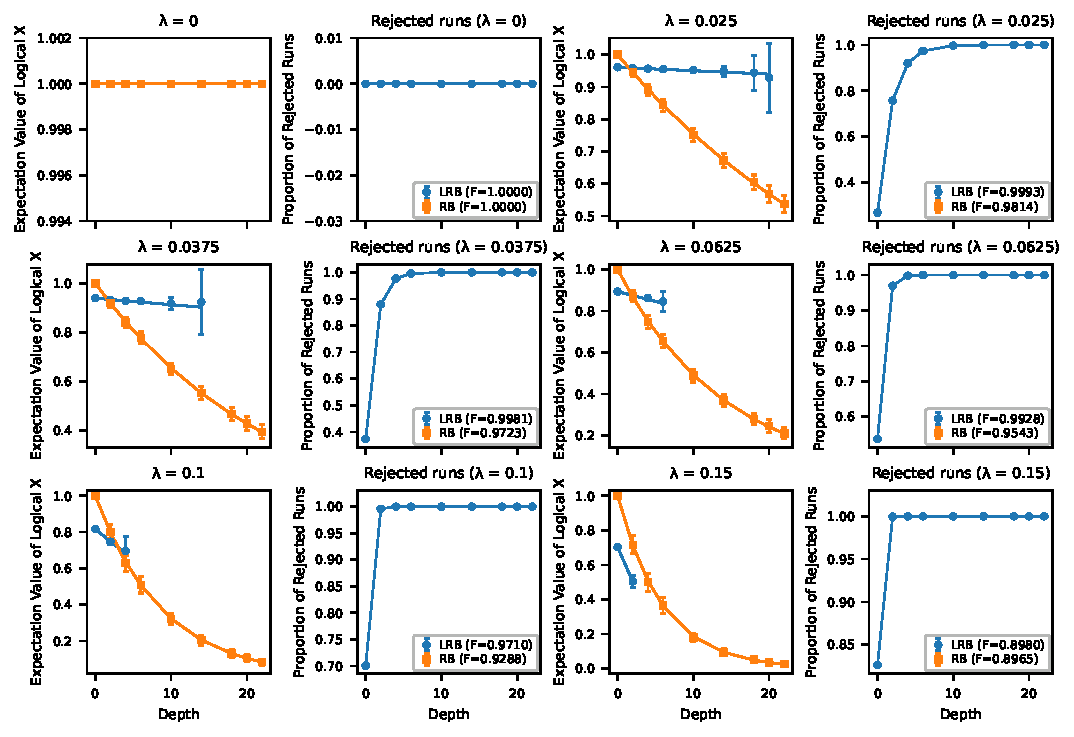
\includegraphics[width=0.95\textwidth]{
    figures/si1000-unif-1-Summary-Graph-Fit.pdf}
  \caption{Uniform interval $k=1$ under qutrit SI1000 noise. Frequent stabilizer filtering restores a single-exponential decay for LRB-D, and the fitted logical fidelities \texttt{F} show a clear improvement over the matched physical baseline below the pseudo-threshold. The noisy check layers make the acceptance cost front-loaded, with substantial rejection already at depth zero.}
  \label{fig:si1000_unif1_fit}
\end{figure}

\paragraph{Intermediate intervals ($k=2,3,4$).}
Spacing the checks out, shown in \autoref{fig:si1000_unif2_fit}, \autoref{fig:si1000_unif3_fit}, and \autoref{fig:si1000_unif4_fit}, trades acceptance for fit quality in the same way as in the depolarizing model. Single-exponential fits remain usable across most of the sweep, with small deviations growing as $k$ increases and more decay modes become accessible between projections. The deviations grow more slowly with $k$ than they did under depolarizing noise, which again reflects how little error the SI1000 model injects between check layers at fixed $\lambda$. As before, we restrict quantitative fitting and threshold extraction to $k \le 4$, and beyond this range the traces develop the same strongly non-exponential features seen in the depolarizing sweeps.

\begin{figure}[H]
  \centering
  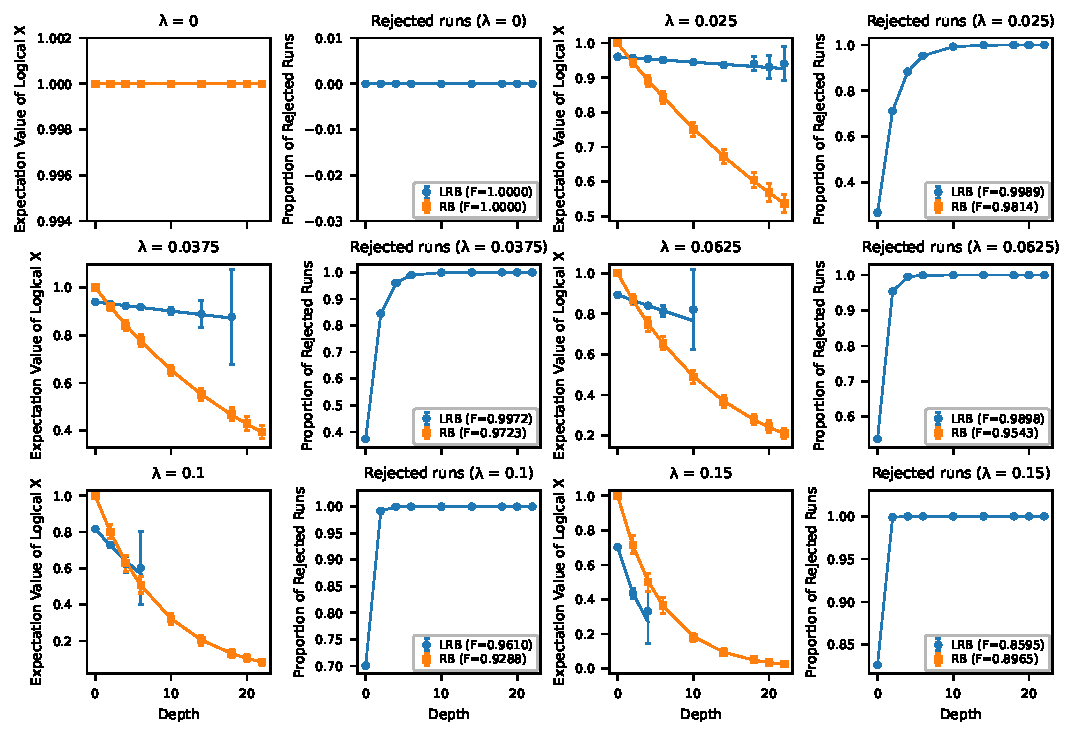
\includegraphics[width=0.95\textwidth]{
    figures/si1000-unif-2-Summary-Graph-Fit.pdf}
  \caption{Uniform interval $k=2$ under qutrit SI1000 noise. Halving the check frequency improves acceptance while the fits remain close to single-exponential.}
  \label{fig:si1000_unif2_fit}
\end{figure}

\begin{figure}[H]
  \centering
  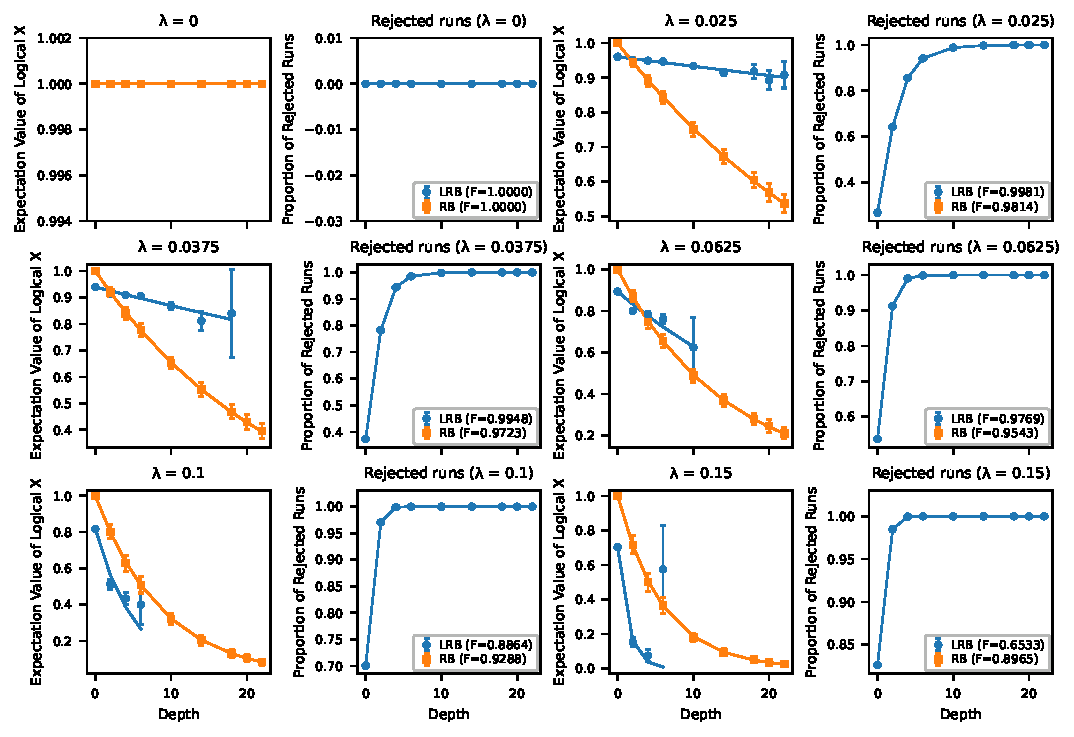
\includegraphics[width=0.95\textwidth]{
    figures/si1000-unif-3-Summary-Graph-Fit.pdf}
  \caption{Uniform interval $k=3$ under qutrit SI1000 noise. Mild multi-mode contamination becomes visible in the extracted decays as the interval grows.}
  \label{fig:si1000_unif3_fit}
\end{figure}

\begin{figure}[H]
  \centering
  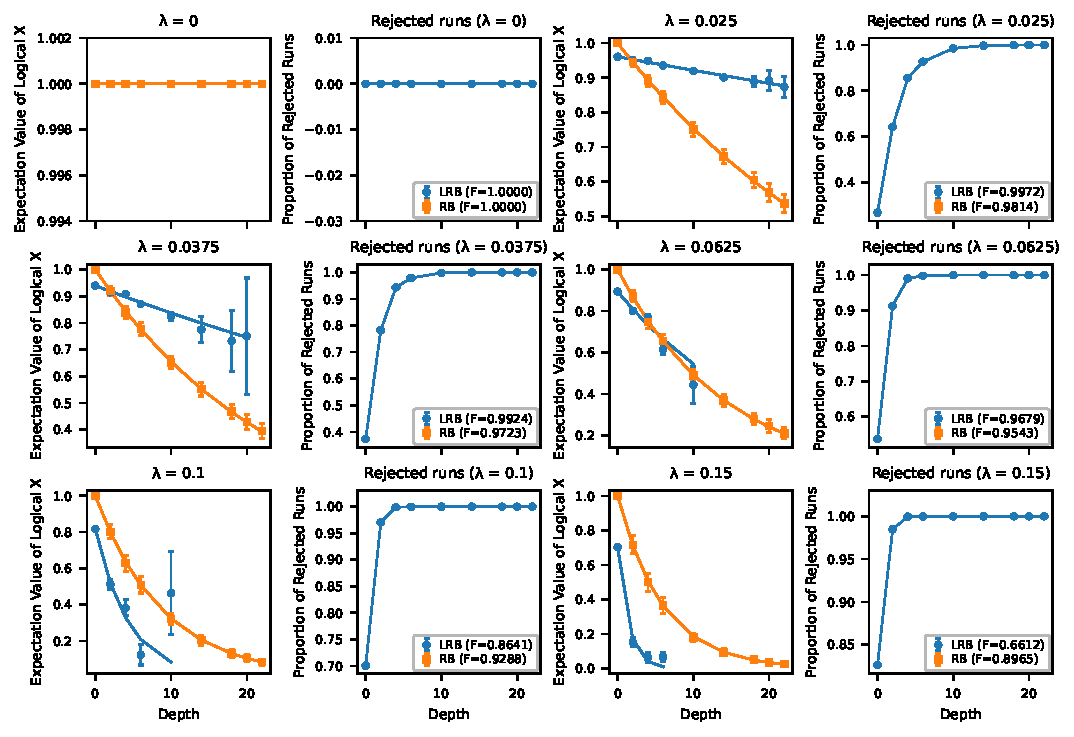
\includegraphics[width=0.95\textwidth]{
    figures/si1000-unif-4-Summary-Graph-Fit.pdf}
  \caption{Uniform interval $k=4$ under qutrit SI1000 noise. As in the depolarizing model this is a practical compromise, with better yields than $k=1$ and decays that are still close enough to exponential to fit.}
  \label{fig:si1000_unif4_fit}
\end{figure}

\subsubsection{Pseudo-thresholds}
\autoref{fig:si1000_threshold_panels} repeats the pseudo-threshold construction of \autoref{sub:simulation_results} on the SI1000 interval-check data, plotting the LRB-D error rate fitted for each uniform check interval at coordinate $\lambda$ against the fitted physical RB error rate at $p_{RB} = \lambda$ and defining $\lambda^\star(k)$ by their intersection. Error bars on the fitted rates are 68\% bootstrap intervals over 500 resamples, and threshold uncertainties use 1000 bootstrap resamples. For the folded patch we find
$\lambda^\star(1) \approx 0.150569 \pm 0.002474$,
$\lambda^\star(2) \approx 0.123274 \pm 0.001336$,
$\lambda^\star(3) \approx 0.079668 \pm 0.000573$,
and $\lambda^\star(4) \approx 0.072530 \pm 0.000871$,
where the quoted uncertainties are bootstrap standard deviations. The bootstrap intervals are mildly asymmetric, for example the 68\% interval for $\lambda^\star(1)$ is $[0.1473, 0.1520]$.

\begin{figure}[H]
  \centering
  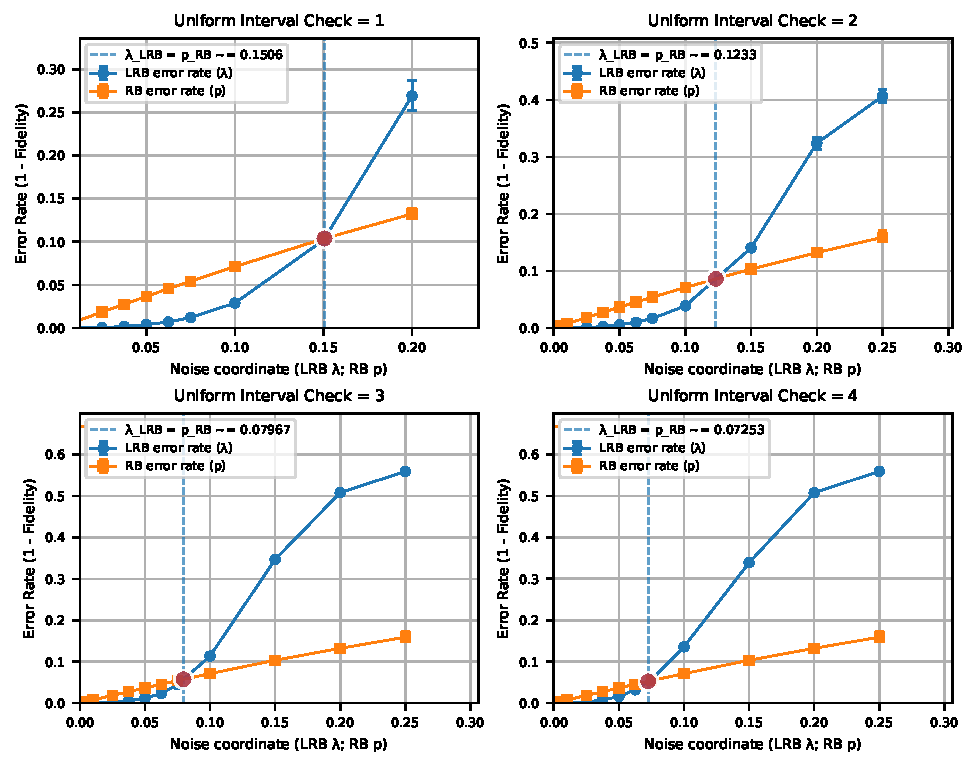
\includegraphics[width=\textwidth]{figures/si1000-unif-threshold-error-vs-p-paper-grid.pdf}
  \caption{Pseudo-threshold construction under qutrit SI1000 noise for uniform check intervals $k=1,2,3,4$. Fitted LRB-D error rates at coordinate $\lambda$ are compared against fitted physical RB error rates at $p_{RB}=\lambda$, and $\lambda^\star(k)$ is defined by their intersection. The RB baseline is linear in $p_{RB}$ as expected for the depolarizing channel, while the LRB-D error rates rise steeply once the check layers and entangling gates dominate.}
  \label{fig:si1000_threshold_panels}
\end{figure}

The trend with $k$, summarized in \autoref{fig:si1000_threshold_trend}, is instructive when placed next to the depolarizing results. At $k=1$ the SI1000 pseudo-threshold sits below the depolarizing value of $p^\star(1) \approx 0.187$, which we attribute to the check layers themselves. Under SI1000 the ancilla readouts are the noisiest locations in the circuit, so checking after every logical gate maximizes exposure to exactly the operations the model penalizes most. For $k \ge 2$ the ordering reverses, with the SI1000 thresholds at $0.123$, $0.080$, and $0.073$ sitting above their depolarizing counterparts of $0.115$, $0.070$, and $0.058$. With so little noise accumulating between checks, spacing the projections out costs less than it does under depolarizing noise, and the decline of $\lambda^\star(k)$ with $k$ is correspondingly shallower. From $k=1$ to $k=4$ the threshold falls by a factor of about $2.1$ under SI1000 compared to about $3.2$ under depolarizing noise.

\begin{figure}[H]
  \centering
  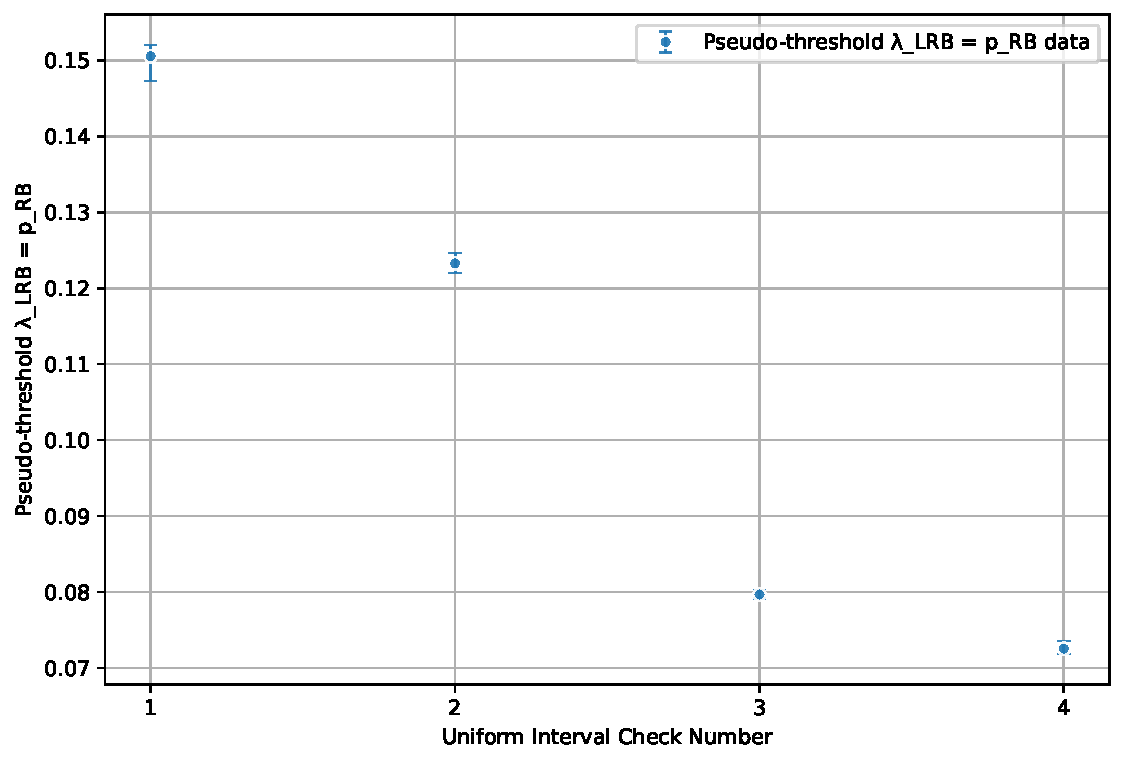
\includegraphics[width=0.65\textwidth]{
    figures/si1000-unif-1-to-4-pseudo-threshold-vs-interval-check-fit.pdf}
  \caption{Pseudo-threshold versus check interval under qutrit SI1000 noise. The threshold decreases as checks become less frequent, but more slowly than in the depolarizing model, since the SI1000 rate hierarchy concentrates the noise in the check layers rather than in the logical gates between them.}
  \label{fig:si1000_threshold_trend}
\end{figure}

The acceptance overhead deserves the same caveat as before. Because the check layers are the dominant noise locations, uniform-interval post-selection under SI1000 rejects aggressively, and past moderate $\lambda$ the accepted fraction at $k=1$ collapses within a few logical gates. The $10^6$ shots per depth point provided by the DEM backend are what keep the accepted-shot statistics usable deep into the sweep. The conditional interpretation of LRB-D discussed at the end of \autoref{sub:simulation_results} carries over unchanged.
